% =====================================================================
%  fig-comparison-groups.tex  —  editable TikZ source for the Background
%  figure "Who the study compares".
%
%  A simplified, schematic version of Fig. 1 in Baylis, Boomhower, Colmer
%  & Voorheis (2026) (the 2020 Glass Fire map). It carries the intuition
%  behind the research design explained in "The challenge": inside one
%  fire perimeter some homes burn and some survive, and a ring of nearby
%  homes just outside the perimeter serves as the comparison group.
%
%  NOT A MAP. Perimeter shape and home positions are invented for
%  illustration — no coordinates from the paper or its data are used.
%  The figure is labelled as a schematic so it cannot be mistaken for
%  the paper's Glass Fire panel.
%
%  Colours and type (Source Sans 3) follow the data-viz design system;
%  hex values are the canonical tokens from
%  formats/research-highlight/_style.tex.
%
%  LAYOUT: sized to sit as tight in its wrap column as the EPA highlight's
%  Background figure — canvas ~154x89mm (aspect ~1.73, matching that
%  figure's 1.75), with the diagram running edge to edge rather than
%  floating inside empty margins. Keep the aspect near 1.75 when editing:
%  at width=3.85in it sets how many lines of Background wrap alongside.
%
%  BUILD (writes the vector PDF into ../figures/):
%      pdflatex -output-directory=../figures fig-comparison-groups.tex
%      rm -f ../figures/fig-comparison-groups.aux ../figures/fig-comparison-groups.log
%  The research highlight reads the PDF from ../figures/, so no copy
%  step is needed — rebuild here and re-render the .qmd.
%
%  To edit: move the home dots, reshape the perimeter, or change the
%  legend wording below and rebuild.
% =====================================================================
\documentclass[border=0pt]{standalone}
\usepackage[T1]{fontenc}
\usepackage[default]{sourcesanspro}   % same typeface as the document
\renewcommand{\familydefault}{\sfdefault}
\usepackage{microtype}
\usepackage{tikz}

% ---- palette (canonical tokens, _style.tex + data-viz guide) --------
\definecolor{ink}{HTML}{1D2620}       % homes that survived (darkest mark)
\definecolor{accentred}{HTML}{641111} % the one emphasis colour: destroyed
\definecolor{muted}{HTML}{50534A}     % structural labels, schematic note
\definecolor{cite}{HTML}{6E6D61}      % legend descriptors
\definecolor{faint}{HTML}{9A978A}     % nearby homes outside the fire
\definecolor{axis}{HTML}{C4BDAD}      % dashed nearby-area boundary
\definecolor{band}{HTML}{F3E4E2}      % pale red tint inside the perimeter

\begin{document}
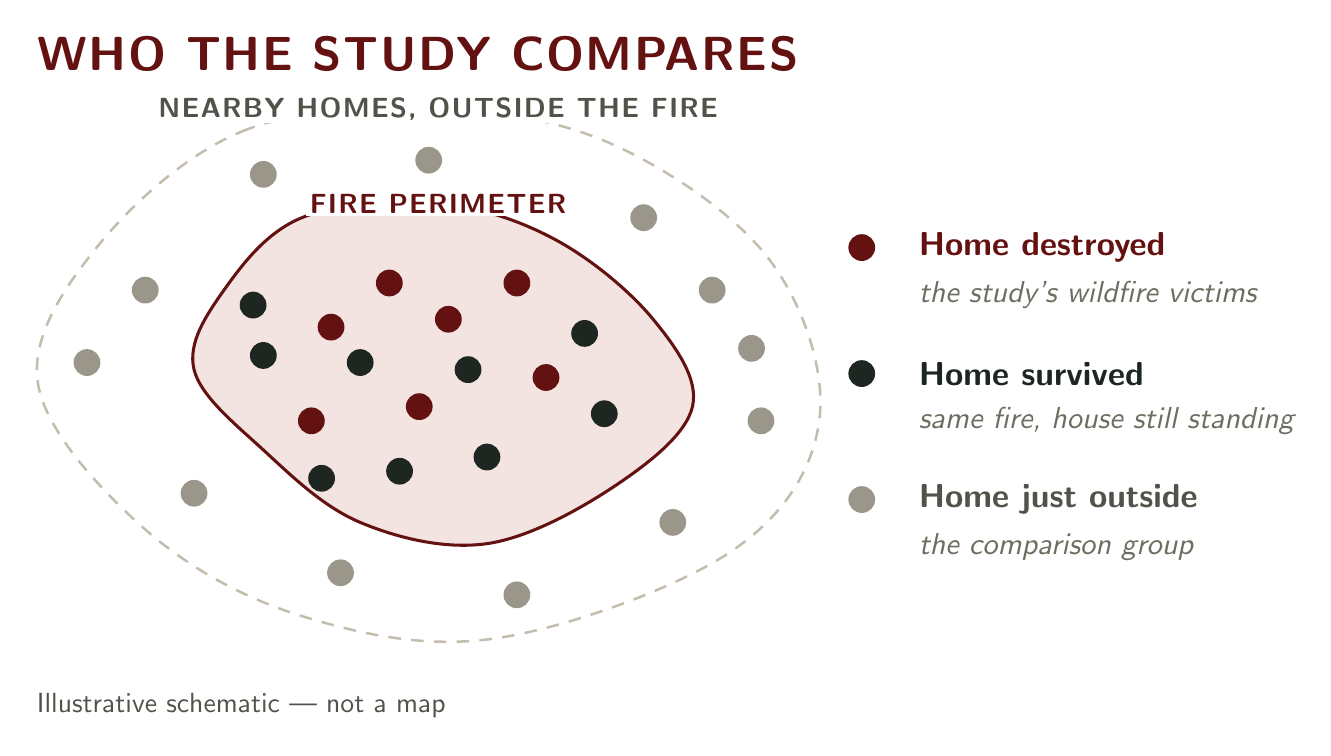
\begin{tikzpicture}[x=1mm,y=1mm,
  dDot/.style={circle, fill=accentred, draw=none, inner sep=0pt,
               minimum size=3.4mm},
  sDot/.style={circle, fill=ink,       draw=none, inner sep=0pt,
               minimum size=3.4mm},
  aDot/.style={circle, fill=faint,     draw=none, inner sep=0pt,
               minimum size=3.4mm},
  onLine/.style={fill=white, inner sep=1.2pt,
                 font=\bfseries\fontsize{10pt}{11pt}\selectfont},
  legLab/.style={anchor=west, font=\bfseries\fontsize{12.5pt}{13.5pt}\selectfont},
  legSub/.style={anchor=west, text=cite, font=\itshape\fontsize{10.5pt}{11.5pt}\selectfont}]

  % --- title (flush left, sits on the canvas edge) ---------------------
  \node[anchor=north west, accentred,
        font=\bfseries\fontsize{17pt}{18pt}\selectfont]
    at (0,89) {\textls[30]{WHO THE STUDY COMPARES}};

  % --- nearby area: dashed boundary outside the fire ------------------
  %  Both outlines use many control points at uneven radii so the smoothing
  %  keeps an irregular, burn-scar shape rather than rounding to an ellipse.
  %  The ring runs to the canvas edges (x~1-101, y~11-79) so the diagram
  %  fills its column instead of floating in white space.
  \draw[axis, line width=0.9pt, dashed, dash pattern=on 1.6mm off 1.3mm]
    plot[smooth cycle, tension=0.6]
    coordinates {(8.9,61.1) (27.4,75.8) (52.2,78.6) (74.6,74.0) (94.4,59.3)
                 (100.6,39.0) (89.4,22.4) (59.7,11.4) (34.9,14.2)
                 (15.0,25.2) (1.4,43.6)};

  % --- fire perimeter -------------------------------------------------
  \draw[accentred, line width=1.1pt, fill=band]
    plot[smooth cycle, tension=0.6]
    coordinates {(25.0,55.6) (34.9,64.8) (52.2,66.6) (67.1,62.0) (79.5,51.9)
                 (84.5,40.8) (74.6,30.7) (58.4,23.4) (42.3,26.1)
                 (30.0,35.3) (21.2,45.5)};

  % --- homes just outside the fire (comparison group) ------------------
  \node[aDot] at (15.0,55.6) {}; \node[aDot] at (30.0,70.3) {};
  \node[aDot] at (51.0,72.1) {}; \node[aDot] at (78.3,64.8) {};
  \node[aDot] at (87.0,55.6) {}; \node[aDot] at (93.2,39.0) {};
  \node[aDot] at (82.0,26.1) {}; \node[aDot] at (62.2,16.9) {};
  \node[aDot] at (39.8,19.7) {}; \node[aDot] at (21.2,29.8) {};
  \node[aDot] at (7.6,46.4)  {}; \node[aDot] at (92.0,48.2) {};

  % --- homes inside the perimeter that survived ------------------------
  \node[sDot] at (30.0,47.3) {}; \node[sDot] at (42.3,46.4) {};
  \node[sDot] at (56.0,45.5) {}; \node[sDot] at (70.8,50.1) {};
  \node[sDot] at (58.4,34.4) {}; \node[sDot] at (47.3,32.6) {};
  \node[sDot] at (37.4,31.7) {}; \node[sDot] at (73.3,39.9) {};
  \node[sDot] at (28.7,53.7) {};

  % --- homes inside the perimeter that were destroyed -------------------
  \node[dDot] at (38.6,50.9) {}; \node[dDot] at (46.0,56.5) {};
  \node[dDot] at (53.5,51.9) {}; \node[dDot] at (62.2,56.5) {};
  \node[dDot] at (49.8,40.8) {}; \node[dDot] at (65.9,44.5) {};
  \node[dDot] at (36.1,39.0) {};

  % --- labels sitting on the two boundaries ----------------------------
  %  White backing plates break the lines they sit on, so keep nearby home
  %  dots clear of their width (~28mm and ~52mm respectively).
  \node[onLine, text=accentred] at (52.2,66.6) {\textls[40]{FIRE PERIMETER}};
  \node[onLine, text=muted]     at (52.2,78.6) {\textls[40]{NEARBY HOMES, OUTSIDE THE FIRE}};

  % --- legend (rows centred on the diagram's vertical span) -------------
  \def\lx{106}\def\tx{112}
  \node[dDot] at (\lx,61) {};
  \node[legLab, text=accentred] at (\tx,61) {Home destroyed};
  \node[legSub]                 at (\tx,55) {the study's wildfire victims};

  \node[sDot] at (\lx,45) {};
  \node[legLab, text=ink] at (\tx,45) {Home survived};
  \node[legSub]           at (\tx,39) {same fire, house still standing};

  \node[aDot] at (\lx,29) {};
  \node[legLab, text=muted] at (\tx,29) {Home just outside};
  \node[legSub]             at (\tx,23) {the comparison group};

  % --- schematic note ---------------------------------------------------
  %  No EIL source line here: the figure is a diagram of the study design,
  %  not a chart of its data, and the page masthead already brands it. The
  %  note stays so the diagram is never mistaken for the paper's map.
  \node[anchor=south west, text=muted, font=\fontsize{10pt}{12pt}\selectfont]
    at (0,0) {Illustrative schematic --- not a map};

\end{tikzpicture}
\end{document}
